\subsubsection{Group Permissions}

Group permissions extend the above system for individual permissions and require the use of smart contracts.

Whilst our application is intended to be fully decentralised, the key stakeholders for some applications (such as health care) may require access to the network to administrate. One example of this is the involvement of the GMC in validating doctor identities. If a doctor has not been registered, or has been struck off, they should not have any access to patient data (even if they claim to be a doctor). They should only have access should the GMC validate that they are in fact a valid doctor.

The idea of a group administrator, such as the GMC, conflicts with the idea of the data owner maintaining full access control and administration. However, should the data owner decide that the group should no longer have any access or wishes to change group permissions, they are able to do so.

To facilitate this, let's take a look at the architecture of a group's interactions with a particular identity's contract.

\begin{figure}[H]
  \centering
  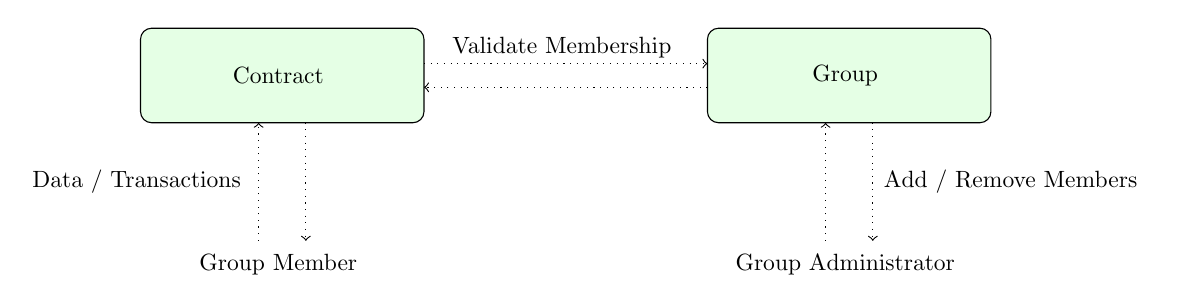
\begin{tikzpicture}[scale = 0.6, every node/.style={scale = 0.85}, every node/.append style={fill = white, rounded corners = 2pt, inner sep = 2pt, align = center}]

  \draw [rounded corners, fill=green!10] (-3, 1) rectangle (3, -1);
  \node [fill=green!10] at (0, 0) { Contract };

  \node at (-3, -2.25) { Data / Transactions };
  \draw [ -> , dotted] (-0.5, -3.5) -- (-0.5, -1);
  \draw [ -> , dotted] (0.5,  -1) -- (0.5,  -3.5);

  \node at (0, -4) { Group Member };

  \draw [rounded corners, fill=green!10] (9, 1) rectangle (15, -1);
  \node [fill=green!10] at (12, 0) { Group };

  \node at (15.5, -2.25) { Add / Remove Members };
  \draw [ -> , dotted] (11.5, -3.5) -- (11.5,    -1);
  \draw [ -> , dotted] (12.5,   -1) -- (12.5,  -3.5);

  \node at (12, -4) { Group Administrator };

  \node at (6, 0.6) { Validate Membership };
  \draw [ -> , dotted] (3,  0.25) -- (9,  0.25);
  \draw [ -> , dotted] (9, -0.25) -- (3, -0.25);

  \end{tikzpicture} \\
  \caption{
  	How a group interacts with an identity's data
  }
  \label{fig:archi_group_interactions}
\end{figure}

